%%%%%%%%%%%%%%%%%%%%%%%%%%%%%%%%%%%%%%%%%%%%%%%%%%%%%
%		INTRODUCCION
%%%%%%%%%%%%%%%%%%%%%%%%%%%%%%%%%%%%%%%%%%%%%%%%%%%%%

\section[Introducci\'on]{Introducci\'on}
\subsection{Vidrios Met\'alicos}

\tikzstyle{every picture}+=[remember picture]

\begin{frame}
\frametitle{Vidrios Met\'alicos (Metal Amorfo)}

\tikzstyle{na} = [baseline=-.5ex]

\centering
\tikz[baseline]{\node[fill=gray!20,anchor=base] (t1){Vidrio};} \tikz[baseline]{\node[fill=gray!20,anchor=base] (t2){Met\'alico};}

\vspace{0.2cm}

\begin{columns}
  \begin{column}{0.48\paperwidth}
    \tikz[na]{\node[coordinate] (n1){};}
    \centering
    \begin{block}{Vidrio}
      \centering Estructura amorfa
      
      \vspace{0.2cm}
      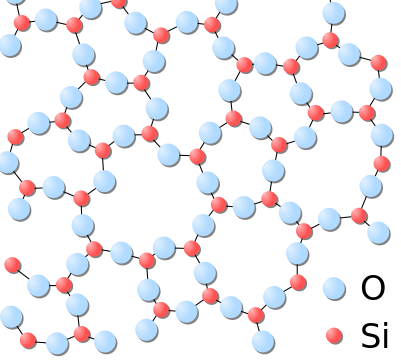
\includegraphics[width=3cm]{../Figures/Cap_1/500px-Silica.png}
    \end{block}
  \end{column}
  \begin{column}{0.48\paperwidth}
    \tikz[na]{\node[coordinate] (n2) {};}
    \centering
    \begin{block}{Met\'alico}
      \centering Aleaci\'on met\'alica:\\
      Cu, Ni, Fe, Au, Zr, Be, La, Pd, Ti\\
      
      \vspace{0.2cm}
      Aunque tambi\'en puede contener no metales en baja concentraci\'on
    \end{block}
  \end{column}
\end{columns}

\begin{tikzpicture}[overlay]
        \path[->] (t1) edge [bend right] (n1);
        \path[->] (t2) edge [bend left] (n2);
\end{tikzpicture}

% \item Sus propiedades sobresalientes los hacen candidatos para aplicaciones modernas y de alta tecnolog\'ia. Material avanzado
\end{frame}

\definecolor{goodTitle}{HTML}{4D9A63}
\definecolor{goodDesc}{HTML}{A0DB8E}
\definecolor{alertTitle}{HTML}{FF2222}
\definecolor{alertDesc}{HTML}{FF9090}

\newcommand{\defaultBlocks}{
  \setbeamercolor{block title}{fg=white, bg=hsrmWarmGreyDark}
  \setbeamercolor{block body}{parent=palette secondary}
  \setbeamercolor{block title example}{fg=white, bg=hsrmSec1Dark}
  \setbeamercolor{block body example}{fg=white, bg=hsrmSec1}
  \setbeamercolor{block title alerted}{fg=white, bg=hsrmRedDark}
  \setbeamercolor{block body alerted}{fg=white, bg=hsrmRed}
}

\newcommand{\ventaja}[2]{
  \setbeamercolor{block title}{bg=goodTitle,fg=white}%
  \setbeamercolor{block body}{bg=goodDesc,fg=black}%
  \only<#1>{
    \begin{block}{Ventaja}%
    #2
    \end{block}%
   }
  \defaultBlocks%
}

\newcommand{\desventaja}[2]{
  \setbeamercolor{block title}{bg=alertTitle,fg=white}%
  \setbeamercolor{block body}{bg=alertDesc,fg=black}%
  \only<#1>{
    \begin{block}<#1>{Desventaja}%
    #2
    \end{block}%
   }
  \defaultBlocks%
}


\begin{frame}
\frametitle{Propiedades}
\begin{block}{¿Por qu\'e atrae el inter\'es de investigadores?}
 Combina propiedades de cer\'amicas y de metales a escala nanom\'etrica, resultando en un material de propiedades \'unicas
\end{block}

\begin{overprint}
 
\ventaja{1}{Ausencia de efectos adversos debidos a fronteras de granos}
\desventaja{1}{Alto costo y grandes limitaciones de fabricaci\'on}
    
\ventaja{2}{Alta dureza. Resistencia al desgaste y la abrasi\'on. Gran resistencia mec\'anica y menor rigidez que las aleaciones cristalinas. Alta resiliencia}
\desventaja{2}{Gran p\'erdida de ductilidad ante la aparici\'on de bandas de corte. El recocido lo vuelve fr\'agil}

\ventaja{3}{Resistencia a la corrosi\'on debido a la falta de bordes de grano}
\ventaja{3}{Algunos MG son biocompatibles}

\end{overprint}
\end{frame}

\begin{frame}
 \frametitle{Algunas aplicaciones de Vidrios Met\'alicos}
 
 \begin{figure}
 \centering
 \begin{tabularx}{\textwidth}{ccc}
 \only<1>{
 \subfloat[Filo est\'andar]{
    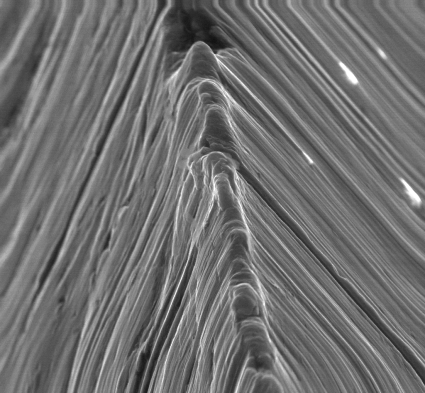
\includegraphics[width=3cm]{../Figures/Cap_1/blade.png}}
  &
  \subfloat[Filo de BMG]{
    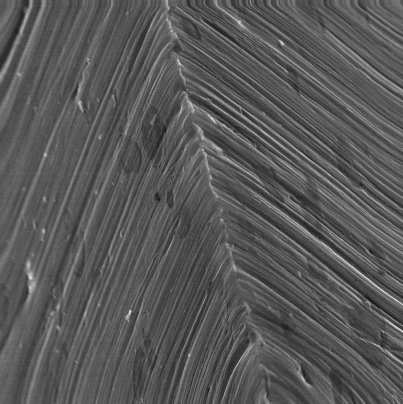
\includegraphics[width=3cm]{../Figures/Cap_1/BMG-blade.png}}
  &
  \subfloat[Joyer\'ia]{
    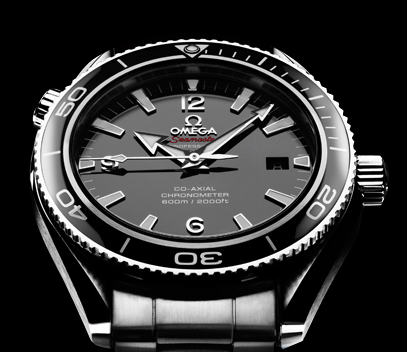
\includegraphics[width=3cm]{../Figures/Cap_1/seamaster.png}}
  }
  \only<2>{
  \subfloat[Deportes]{
    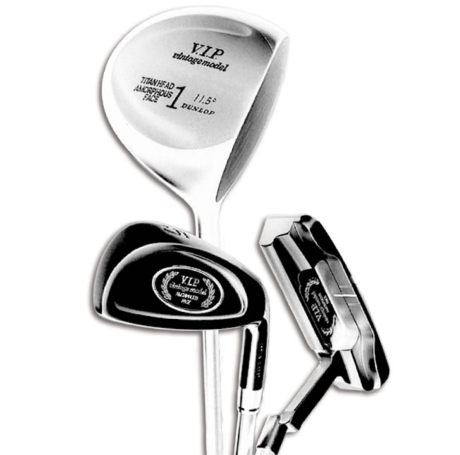
\includegraphics[width=3cm]{../Figures/Cap_1/golf.png}}
  &
  \subfloat[MEMS]{
    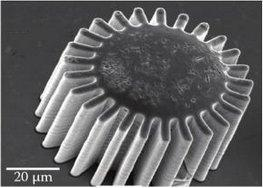
\includegraphics[width=3cm]{../Figures/Cap_1/MEMS_A.jpeg}}
  &
  \subfloat[MEMS]{
    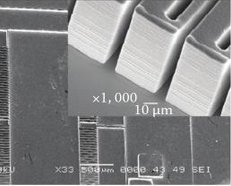
\includegraphics[width=3cm]{../Figures/Cap_1/MEMS_B.jpeg}}
    }
 \end{tabularx}
\end{figure}
\end{frame}

